Distance based methods are probably the simplest way to classify time series. They rely on a measure function that relates the time series to a single numeric value which indicates the similarity between two different time series. Then, a classification method can be used to separate different classes of time series. \cite{Xing10}

In this chapter I first present $L_p$ norms and Dynamic Time Warping (DTW) as examples of measure functions. Then, k-nearest neighbors (kNN) and learning vector quantization (LVQ) algorithms are formulated for classifying the time series.



\subsection{$L_p$ norms}
One way to classify time series is to calculate a distance measure between a new time series and the existing labeled time series. Then, one can select the group with has the lowest distance with the time series being classified. The easiest approach is some $L_p$ norm which can be calculated for time series $\mathbf{x} = \{x_0, x_1, ..., x_{n-1}\}$ and $\mathbf{y} = \{y_0, y_1, ..., y_{n-1}\}$ with \cite{smith07}

\begin{equation}
D(\mathbf{x}, \mathbf{y}) = \left( \sum_{i=0}^{n-1} \left| x_i - y_i \right|^p \right)^{\frac{1}{p}}.
\end{equation}

Then, one can use various algorithms, such as nearest neighbor classifiers or decision trees, to classify the time series into different groups. Examples of $L_p$ norms are Manhattan norm ($p = 1$), Euclidean norm ($p = 2$) and maximum norm ($p \rightarrow \infty$). $L_p$ norms are very straightforward to calculate but requires normalization of the signals in order to handle similar signals with different amplitudes. \cite{MiningTimeSeriesData} 

\subsection{Dynamic Time Warping}
$L_p$ norms cannot group signals that are, for example, in different phases, no matter how similar they are. One way to overcome this problem is to use dynamic time warping (DTW) algorithm. It measures the similarity between two signals that may vary in time or speed by "warping" the axis of one time series so that the phases of the signals match. \cite{MiningTimeSeriesData} Let us denote a feature space, that is, available values for $x_i$ and $y_j$ by $\digamma$. A classical DTW algorithm begins by creating a matrix 

\begin{equation}
C(i, j) = c(x_i, y_j),
\end{equation}
where $c$ is a local distance measure: $c \ : \ \digamma \times \digamma \rightarrow \mathbb{R}$ that is the difference between the two variables. In other words, the two time series being compared are laid on the two axes of the matrix and the matrix contains the differences between the corresponding values in the time series.

Then, by using dynamic programming, a monotonically increasing minimal path from the bottom left corner of the matrix to the top right corner is searched. The algorithm begins by calculating the cumulative matrix \emph{D} beginning from the bottom left corner of the cost matrix \emph{C}. Then, the minimum path in the cumulative matrix defines the optimal alignment between \emph{x} and \emph{y}. \cite{Muller07} 

The difference between Euclidean distance and DTW distance is illustrated in Figure~\ref{fig:euclidean_vs_dtw}. While Euclidean distance always compares the two time series point by point, DTW distance warps the other time series so that the extrema of the two time series are matched. This gives a more comprehensive similarity measure for two time series.

\begin{figure}[here]
\centering
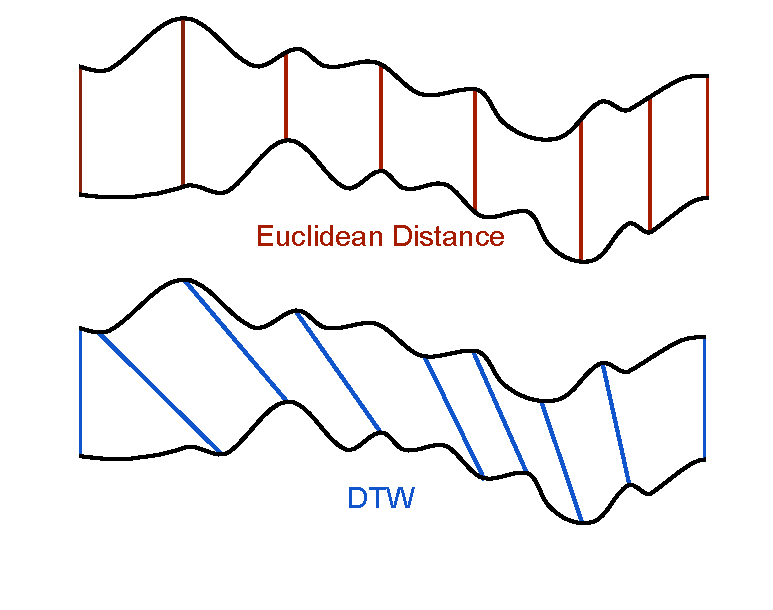
\includegraphics[scale=0.7]{images/euclidean_vs_dtw.pdf}
\caption{Difference between Euclidean Distance and Dynamic Time Warping.}
\label{fig:euclidean_vs_dtw}
\end{figure}



The vertical lines in the figure illustrate the points in the time series that are compared against each other. As can be seen, the algorithm matches the peaks and the valleys with one another. A pseudo code is presented in the following:


\begin{algorithm}[H]
	\KwData{Cost function $c$, Width $N$, Height $M$}
	\KwResult{Optimal Warping Path $p$}	
	Calculate cumulative cost matrix D starting from bottom left corner\;
	Set n = N and m = M\;
	\While{n > 0 and m > 0}{
		Move to neighbor with the smallest D(n, m)\; 
		Store movement to p\;
		Update n and m\;
	}
	reverse $p$\;
	return $p$;
\end{algorithm}


\subsection{k-Nearest Neighbor Algorithm}
Our classifying task consists of two classes as shown in Equation~\ref{eq:classification}. Once we have agreed on which distance measure we are using, we can use k-nearest neighbor (kNN) algorithm to classify new time-series instances. In the experimental chapter of this thesis I use Dynamic Time Warping (DTW) that was introduced in the previous section.

The kNN algorithm is a supervised learning algorithm, which means that we need a labeled teaching set to initialize the algorithm. \cite{PatternRecognition} The time-series in the teaching set have been labeled so that their label is either $w_1$ or $w_2$ depending on which class they belong to. 

Now for every new time-series instance we calculate the distance between the new instance and all the instances in the teaching set. Then, we select the $k$ instances with the least distances to our new instance. These $k$ instances vote for how the new instance is classified: the class with most instances is chosen. Clearly, the parameter $k$ should be odd so that we avoid draws between the two classes. \cite{Hastie08}


\subsection{Learning Vector Quantization}
Learning vector quantization (LVQ) is a supervised neural network that uses winner-take-all prototype-based learning. The LVQ algorithm, first developed by Teuvo Kohonen \cite{Kohonen90}, is similar to the kNN except for the application of moving prototype vectors. The M prototype vectors $\{z_1, ..., z_M\}$ are labeled vectors that represent the classes $C(z_m), m = 1, 2, ..., M$ and can be selected randomly from the set of available training vectors. Then, for each training vector $x_i, i = 1, ..., N$ the nearest prototype vector $z_m$ is updated with the following rule:
\begin{align}
z_m \leftarrow 
\begin{cases}
z_m + \alpha (x_i - z_m), & \text{if $z_m$ and $x_i$ belong to the same class} \\
z_m - \alpha (x_i - z_m), & \text{if $z_m$ and $x_i$ belong to different classes}
\end{cases},
\end{align} 

where $\alpha$ is the learning rate. In other words, the closest prototype vector is moved towards the instance if its from the same class as the prototype vector. In the opposite case, the prototype vector is moved away from the instance. When using the model with testing data, each new instance is classified with the same class as the closest prototype vector.

Usually, the training vectors are iterated through multiple times for a better convergence. On every iteration the value of $\alpha$ can be decreased so the algorithm first takes larger steps and then gradually moves to smaller steps. By doing this it first moves the prototype vectors to correct areas and then refines their positions. \cite{Li08}

